\documentclass[11 pt,a4paper]{article}
\pdfoutput=1
\usepackage{gensymb}
\usepackage[utf8]{inputenc}
\usepackage[T1]{fontenc}
\usepackage[swedish]{babel}
\usepackage{amsmath} 
\usepackage{lmodern}
\usepackage{units}
\usepackage{icomma}
\usepackage{tikz}
\usepackage{pgf-pie}
\usepackage{color}
\usepackage[dvipsnames]{xcolor}
\usepackage{graphicx,caption}
\usepackage{hyperref}
\usepackage{filecontents}
\usepackage{subcaption}
\usepackage{bbm}
\usepackage{todonotes}
\usepackage{pdfpages}
\usepackage{float}
\usepackage[utf8]{inputenc}
%\usepackage[top=1.4in, bottom=1.3in, left=1.5in, right=1.5in]{geometry}
\usepackage{pgfgantt}
\usepackage{float}


\definecolor{lila}{RGB}{128,0,128} %Ida
%Mahogany - Mattias
%Cyan - Björn
%WildStrawberry - Axel
\definecolor{green}{RGB}{25,150,50} %Påja

\begin{document}

\includepdf{Figures/Framsida.pdf}
%Förslag på ny titel
% Titel: Problemlösningsuppgifter för gymnasiet
%Undertitel: med fokus på verklighetsanknytning, modellering, programmering och diskussion
% 

\pagenumbering{gobble}

\newpage

\renewcommand\abstractname{Sammandrag}\begin{abstract}
\noindent \textcolor{green}{Matematik är ett kärnämne i skolan. Samtidigt är en vanlig upplevelse för många elever att det är svårt, tråkigt och oanvändbart. Med detta projekt ville vi ändra på detta genom att införa nya typer av matematiska problem för gymnasieskolan. Dessa problem låter eleverna arbeta mer med problemlösning. Problemen har en realistisk verklighetsanknytning, ger underlag för diskussion, går att lösa på olika sätt, och ska framför allt ge känslan av att matematik är användbart. Eftersom programmering snart ska införas i skolmatematiken är även en del av problemen konstruerade för att förbereda inför det.}

\textcolor{green}{Som en del av vårt resultat gjorde vi bland annat en undersökning som 58 lärare deltog i. 91\% av lärarna angav att de arbetade för att inkluderade mer problemlösning samtidigt som 42\% tyckte att det var svårt att hitta bra problem. Efter att problemen testades på gymnasieskolor svarade en del av eleverna på en enkät om sin upplevelse av det problem de arbetade med. Av de som svarade angav 80\% att de lärde sig något nytt och 75\% uttryckte på något sätt att problemet var roligt eller meningsfullt.}

\textcolor{green}{Vår slutsats blev att lärare idag vill inkludera mer problemlösning i undervisningen, men att det inte är lätt att hitta bra problem, samtidigt som en del har tidsbrist. Trots att vi inte lyckades testa problemen i så många klasser som vi hade önskat, så var både vi och lärarna som testade dem nöjda med problemen.}
\end{abstract}

\newpage

\renewcommand\abstractname{Abstract}
\begin{abstract} 
\noindent \textcolor{WildStrawberry}{
    Mathematics is a core subject in the Swedish school system. Parallel to this, it is a common occurence that the subject is perceived as hard, boring and useless. With this project we want to faciliate the teachers by introducing new mathematical problems targeted for upper secondary school pupils. We conducted a survey for teachers; where 91\% asserted that they are working to include problem-solving in their teachings, while 42\% have issues finding good problems. The main purpose of this project has then been to produce problems designed to help the teachers in question. The problems are open, applicable to real-life, give ground for discussion and, perhaps most importantly, make mathematics feel relevant. Also, since programming is soon going to be part of mathematics, a share of our problems have been constructed to prepare students for this inclusion. Additionally to these problems, a suggested ''complete'' lesson plan is provided and presented on an easily accessible and user-friendly web page. Finally, from all our tested problems, the 26 student answers assert that: 80\% declare they learnt something new and that 75\% state they found the problem fun or meaningful in some way.
    }
    
    %This project aims to change this by introducing \textit{relevant} and easily accessible problem-solving tasks for upper secondary school pupils.  Thus the main purpose
    
    %These problems are designed to spark initiative and allow for creative solutions. Analogous to the real-world, the problems should encourage discussion whether they can be solved in multiple ways or if solutions can be refined to better model, but perhaps most of all: feel useful. Also, since programming is going to be introduced in school mathematics, some problems are made to test and prepare students for the inclusion of programming. }
    
%\textcolor{WildStrawberry}{
    %As a part of the result from the project, 58 teachers took part of our survey.     After testing our problems, some of the pupils answered a questionnaire regarding their experience when approaching the problems. From the 26 answers: 80\% declared that they learnt something new and 75\% stated that they found the problem fun or meaningful in some way.}
    
%\textcolor{WildStrawberry}{
    %Our conclusion is that teachers want to include problems-solving in their teachings, however finding well made problems isn't an easy task and that they lack the time to craft problems themselves. The reach we surmounted to wasn't huge, but the teachers who did try our problems seemed content.}
\end{abstract}

\newpage
 
\tableofcontents

\newpage
\pagenumbering{arabic}

%\section*{Mall med idéer, fyll gärna på mer}
%    \section{Introduktion}

    \subsection{Matematikundervisningen idag}
    
    \subsection{Förändringar under senare år}
        Här kan man ta upp de förändringar som genomförts hyfsat nyligen: 
        \begin{itemize}
            \item Det arbete som lagts på att införa mer problemlösning och modellering
                \subitem Ändrar i kursplanerna
                \subitem Mattelyftet
            \item Den nya ändringen med programmering
        \end{itemize}
        Man kan avsluta med en diskussion om att förändringarna tar mycket tid och energi m.m. och vad vårat arbete kan göra för att hjälpa till här.
        
\section{Teori}
    Teori om den pedagogik vi använder:
    \begin{itemize}
        \item Diskussioner och kommunikation inom matematik  %Björn
        \item Arbete i grupp? Olika gruppstorlekar? Fördelar/nackdelar? %Björn
        \item Programmering och matematik
    \end{itemize}

\section{Metod}
    \subsection{Skapandet av problemen}
        Hur vi har tänkt

    \subsection{Hemsidan}
    
\section{Resultat}
    \subsection{Problemen}
        På något sätt berätta om (ev. bara några av) de problem vi har skapat.
    
    \subsection{Hemsidan}

\section{Utfall}
    Här kommer svaren på enkäterna (förhoppningsvis)

\section{Diskussion}

\section{Slutsats}


% \section{Bakgrund}
%     \label{sec:Bakgrund}
%      \textcolor{lila}{Avsnittet introducerar projektet, samt de bakomliggande problem som fått oss att vilja sätt oss in i ämnet.}
    
    \section{Matematikundervisning nu och då}
        \textcolor{lila}{Matematik är en av de största delarna i skolan i Sverige idag, vilket bland annat visar sig genom att matematiken är kärnämne i både grundskolan och gymnasiet. Trots det är det ett ämne som många elever blir stressade över, och som ofta framställs som svårt, tråkigt, oanvändbart och abstrakt \cite{Ignacio&Barona}. En vanlig uppfattning verkar också vara att matematik är ett ämne som bara ett fåtal kan bli bra på \cite{Skolverket03} och ett ständigt återkommande inslag i media är det faktum att matematikkunskapen i Sverige har gått ner \cite{CompareOECD}. Men hur ser undervisningen ut idag? Vad kan man ändra för att förbättra dessa resultat?}


        
    \subsection{Traditionell matematikundervisning}
        \textcolor{lila}{Den så kallade traditionella undervisningsmetoden består av två delar: \textsl{genomgång} och \textsl{egen räkning} \cite{traditionellMatte}. Det innebär att lektionen börjar med att läraren står framme vid tavlan och går igenom ny teori varefter varje elev individuellt får träna på detta med hjälp av ett stort antal likartade uppgifter. Därefter kan eleverna kontrollera om de gjort rätt genom att jämföra svaret med facit, och därefter gå vidare. Om man får rätt svar på alla uppgifter anser man sig ha förstått den nya teorin. Därefter upprepas samma procedur med ett nytt begrepp i centrum.} 
    
\textcolor{lila}{Med den här metoden lär sig eleverna olika matematiska begrepp och metoder, men först efter att det specifika begreppet eller metoden just presenterats. På det faktiska provet, när de själva måste ta reda på vilken metod som ska användas i varje uppgift, blir det betydligt svårare \cite{TheElephant}. }
\textcolor{WildStrawberry}{
    Just på grund av detta så tar man ett steg ifrån verklighetskopplingen och användbarheten av matematiken. När applikationen av teorin blir mekanisk istället för modellerande så tappar teorin syftet och blir mer av ett verktyg för att få ut rätt svar från en fråga. Fokus blir att man utnyttjar korrekt formel och snabbt får feedback från facit, eller andra hjälpmedel, om man fått rätt svar istället för att förstå problemet och dess underliggande moment för vad dem faktiskt innebär. }
    
    \subsection{Förändringar i matematikundervisningen}
        %Förändringar i matematikundervisningen

\textcolor{lila}{Den traditionella undervisningen var länge den som mer eller mindre uteslutande användes i Sverige, särskilt i högre åldrar. På senare år har man dock börjat att aktivt se över hur undervisningsmetoden skulle kunna förbättras.}

\textcolor{lila}{År 2011 infördes en ny och uppdaterad kursplan för gymnasiet, GY11, som bland annat påverkade matematiken. Jämfört med de tidigare kursplanerna från 2000 fanns det ett antal viktiga ändringar som gällde alla de olika matematikkurserna. %Ej nytt stycke!
Dels lägger de nya kursplanerna mer fokus på att kurserna ska anpassas efter varje program och inriktning. På så sätt plockas begreppet ''verklighetsanknytning'' upp på ett tydligare sätt. Man ska alltså lära sig hur matematik kan användas i vardagssammanhang som t.ex för att betala räkningar, men även i mer specifika sammanhang beroende på vad du kan behöva i yrkeslivet alternativt vidareutbildningen efter gymnasiet. 
En annan viktig ändring tar upp problemlösning. Detta har ingått även tidigare, men då bara som ett mål utöver de övriga. Nu ska det även användas som medel för inlärning av de andra målen. Kursplanen poängterar nu också att undervisningen ska varieras och innehålla undersökande aktiviteter. \cite{GY00-GY11}}

\textcolor{lila}{För att dessa förändringar ska kunna implementeras på ett så bra sätt som möjligt har man också gjort en stor satsning genom att utbilda alla lärare. Detta har gjorts genom \textsl{Matematiklyftet}, som är en kompetensutveckling i didaktik för lärare. Här belyses den kommunicerande, reflekterande och undersökande delen av matematiken. \cite{Nämnaren}}
            
\textcolor{lila}{Problemlösning är alltså ett mycket aktuellt ämne, som man lägger mycket resurser på att införa i matematikundervisningen. Det är dock en mycket stor förändring att genomföra, och det tar därför tid. Många lärare tycker också att det är svårt att hinna med problemlösning vid sidan av det material som redan ska täckas enligt kursplanen \cite{2016Senare}. Även de lärare som arbetar aktivt med att införa mer problemlösning stöter på problem. Kanske är det för att flesta elever är vana vid den traditionella undervisningen. Eleverna förväntar sig då att lärarna ska tala om precis hur man ska göra och vad som är rätt och fel. De gamla vanorna kan alltså sitta djupt hos både elever och lärare, och vara svåra att ändra.}

\textcolor{lila}{I mars i år (2017) beslutades också att skolan ska verka för att stärka elevernas digitala kompetens \cite{regeringen}. För gymnasiematematiken innebär detta att användingen av digitala verktyg ska bli mer central och programmering ska användas för att lösa matematiska problem \cite{itiskolan}. Även här ska det genomföras fortbildning av lärare \cite{prog_utbildning}.}
            
\textcolor{lila}{Vi har pratat med lärare som saknat tillräcklig hjälp i den här övergången till GY11. Trots den stora satsningen Matematiklyftet, där lärare utbildades om nya tankesätt kring matematikundervisning, så är det svårt att införa problemlösning i en klass som inte arbetat med det tidigare. Det finns gott om bra uppgifter, men det saknas hjälp med \emph{hur} man lär ut problemlösning från början. 
Ett rimligt antagande är att den kommande övergången, till att införa mer programmering och andra digitala verktyg i matematiken, också den kommer bli svår och ta lång tid att genomföra.}
%Ev. avsluta med något mer positivt, t.ecx hur vårt arbete kan hjälpa till
        \label{sec:Forandringar}
        
    \subsection{Verklighetsanknytning i matematiken}
        \textcolor{lila}{En vanlig uppfattning är att det finns för lite verklighetsanknytning i matematiken som lärs ut \cite{TheElephant}. Mot denna bakgrund är det lätt att förstå att elever kan tolka ämnet som onödigt och irrelevant, vilket förklarar varför det är så viktigt att eleverna upplever uppgifterna som relevanta.}

\textcolor{lila}{Detta är ett faktum som många kursboksförfattare tagit fasta på, men tyvärr uppnår dessa försök inte alltid målet. Ofta känns den så kallade verklighetsanknytningen forcerad, och det blir snarare dåligt förklädda matematikuppgifter än faktiska problem som man kan föreställa sig att någon skulle vilja lösa. Detta riskerar att ge eleverna en känsla av att matematik inte är användbart, eftersom de får se så få exempel från dess verkliga användningsområden.
I vissa fall har man också tänkt för mycket på att den relevanta matematiken ska finnas med i uppgiften, vilket kan leda till att rimligheten blir lidande. Jo Boaler beskriver det som att eleverna inser att det finns ett speciellt ''matteland'', där det vanliga sunda förnuftet inte längre gäller. \cite{TheElephant}}
    
\textcolor{lila}{De textuppgifter som skrivs  i kursböcker med avsikt att införa en verklighetsanknytning kan också enligt vår erfarenhet i många fall brytas ner till standardproblem enbart genom att plocka ut siffrorna ur texten. På så sätt kan man också ofta bortse från den verklighetsanknytning som eventuellt finns i uppgifterna.}

\textcolor{lila}{Det verkar alltså vara viktigt med verkligehtsanknytning i matematiken, så att eleverna kan relatera till uppgiften och få känslan av att matematik är viktigt och användbart.}
        
    \subsection{Matematikundervisningen idag}
        \textcolor{WildStrawberry}{
    Den svenska matematikundervisning idag är relativt lik den traditionella matematikundervisningen, i stora drag gäller det att en lärare lär ut ett eller flera teoretiska begrepp inför sin klass och sedan ska klassen repetera dessa nya begrepp \ref{sec:Traditionellt}. }
    
    %Repetitionen i sin tur, kommer troligtvis innebära att eleven sitter med en lärobok som har en mängd definierade uppgifter där den nya teorin ska appliceras. Detta sker ändå trots att skolverket definierat ny läroplan som ska motverka . Detta moment kommer att hamna i en sluten loop tills det är dags för det stora provet där man testar alla begrepp man tidigare gått igenom. 

% <3 miss you <3

%ny rubrik? problemet?
%\textcolor{WildStrawberry}{
 %   Problemet med denna typen av undervisning är att eleven inte behöver känna igen det underliggande problemet, eleven kommer undan med att memorera hur en formel ser ut – utan att nödvändigtvis behöva förstå vad formeln gör. Inte för att testa förmågan att memorera saker är dåligt, men just på grund av detta så tar man ett steg ifrån verklighetskopplingen och användbarheten av matematiken. När applikationen av teorin blir mekanisk istället för modellerande så tappar teorin syftet och blir mer av ett verktyg för att få ut rätt svar från en fråga. Fokus blir att man utnyttjar korrekt formel och snabbt får feedback från facit, eller andra hjälpmedel, om man fått rätt svar istället för att förstå problemet och dess underliggande moment för vad dem faktiskt innebär. }


%vad matematiken & skola bör lära ut

% från intervju med Gymnasieelev när ställd frågan "blir ni skolade på hur man löser problem eller är problemlösningen ett vanligt matteproblem som är maskerat i text?": 
%" Mestadels det senare, vi gör problemlösningen i matten så man ska försöka hitta den användbara infon och lösa matteproblemet. Jag tar lite svårare matte men samma kurs som andra så min grupp får lite mer roliga problem där man måste använda logik i kombination med algebraisk matte...

% Men generellt så löser man mest maskerade matte problem"

\textcolor{WildStrawberry}{
    Enligt den nya läroplanen för matematik, så ska matematiken beröra problemlösning på så vis att man ska lära sig behärska sunt resonemang och logik \ref{sec:Forandringar}. Eleven ska alltså kunna bemöta uppställda situationer med metodik och kunna modellera lösningar från given information. Trots dessa förändringar så verkar det som applikationen av problemlösning i skolan är bristande. Elever får fortfarande uppgifter som är förklädda i en ''kort historia'' där målet egentligen blir läsförståelse över problemlösning . Givetvis låter det bra att ha mer problemlösning, men om inte mycket har förändrats så är försöket ett misslyckande \todo{har vi en bra källa på detta?}. När verklighetsanknytningen känns forcerad eller löjlig så missar man målgruppen. Sanningen blir att matematiken kommer känns mer oanvändbar \ref{sec:Verklighetsanknytning}. Än behöver alltså fler åtgärder vidtas innan man uppnår den typ av kreativ problemlösning som eftersträvas.
    %Från vår undersökning så får elever uppgifter, precis som i läroboken, maskerade i en kort saga som ska simulera ett problem. Reglerna är ofta tydliga och tanken är att man hittar siffrorna i texten och använder korrekt formel som man fått på undervisningen. 
}

\textcolor{WildStrawberry}{
    Nedan finns uppgifter tagna från en matematikbok, \cite{matte5000}, som trycktes 2011, alltså från en bok som är designad utefter förändringarna som ska vara aktuella med GY11.}

% <3<3<3
%(citat från intervju? hittas i .tex filen ovanför stycket).
% HEEEJ :D ändra precis som du könner är swag! jag bara får ut något på papper just nu :)
% Haha, det är bra att du skriver! :D Tänkte bara hjälpa till när jag såg det och kunde :)
% Super! :D All hjälp är toppen, tror du jag tänker rätt på denna sektion? den är ju mycket lik den om traditionell skola
% Ja... Det är jag lite osäker på... Funderar på om det inte är bättre att du försöker lägga in delar av det du skrivit i det stycket... Det är ju också svårt att påstå saker utan källor, så det måste vi försöka vara noga med. 
% AA exakt! Men på sätt och vis har vi en "intervju" med en duktig matte-student. Som är en källa. Dock en källa 
% - intJeo a,l ol skoor.
% wow :D

% Det är nog också mer relevant till "matematiken idag". Det existerar en bekvämlighetsfaktor just på grund av tiden är bristande och därför är det najs att använda sig av färdiga problem som inte har mycket tanke bakom sig. - Eleven får övning och "problemlösning (läsförståelse)"

% :( 
% okej <3 <3<3<3<3 till synes borta :smirk:
% Haha, förlåt xp
% Tänket bara säga att vi ju kan använda det som att vi vet att det händer, men inte som att det alltid är så. Vi kan också gå in mer på att det är svårt att hinna med, och ta in lite mer från planeringsrapporten. Precis, eller inte från lärarnas håll i alla fall ;)
% Ska vi ta bort detta nu kanske :p
%Fixade! ;) Inte helt borta i alla fall!

%Här kommer några bra dåliga problemlösningsuppgifter ifrån \cite{matte5000} - MVH Björn

%Följande är en a uppgift, dvs en lätt uppgift:
\begin{displayquote}
\textcolor{turkos}{Marcus läser en bok som innehåller 420 sidor. Mellan kl 19.45 och 20.15 läser han 14 sidor. \\
Hur lång tid tar det att läsa hela boken?}
\end{displayquote}

%Svar

%Detta är en b-uppgift
\begin{displayquote}
\textcolor{turkos}{Jonas kör sin bil samma sträcka varje dag. Sträckan är en mil och Jonas brukar köra med hastigheten 90 $km/h$ en dag kör han sträckan med 100 $km/h$. \\
Hur många sekunder ''tjänar'' Jonas på det?}
\end{displayquote}

%Svar

%Följande två uppgifter är c-uppgifter, dvs de svåraste. 

\begin{displayquote}
\textcolor{turkos}{Vilket tal är x?\\
\( 2*5^x + 3*5^x = 25^{12} \)}
\end{displayquote}

%Svar

\begin{displayquote}
\textcolor{turkos}{En sandstrand är 2km lång, 30 m bred och 3 m djup. \\
Vi antar att ett sandkort ryms inom ett kubiskt område med sidan 0,2 mm.\\
Hur många sandkorn finns på stranden?}
\end{displayquote}

%Svar

%Samtliga fyra uppgifter har tagits från delkapitel 1.4 Problemlösning, som är del av 1 Aritmetik - Om tal. Finns liknande uppgifter i kapitlen om 2.2 Procentuellea förändringar och 3.2 Linjära ekvationer och olikheter. Dock saknas helt uppgifter om problemlösning för Geometri, Sannolikhetslära och statistik, samt Grafer och funktioner. 

\textcolor{WildStrawberry}{
    Det krävs inte mycket tid för att hitta all information man behöver för att kunna lösa uppgiften. Författaren av uppgifterna har knappt heller försökt testa läsförståelsen av den som löser uppgiften med att slänga in irrelevant data. \todo{lol, savage stycke är savage} Det är möjligt att eleven hade fått mer ut av en färdiguppställd ekvation och mekaniskt fått öva på att bara lösa ut x, och ha mer tid för fler mekaniskt uträknande i uppgifter.}
        
    \subsection{Gruppindelning}
        \label{sec:Gruppindelning}
        \textcolor{cyan} {Det är vanligt att dela upp elever efter hur snabbt de anses lösa uppgifter. Elever som löser uppgifter snabbt grupperas med andra elever som löser uppgifter ungefär lika snabbt, och det samma gäller elever som anses lösa uppgifter långsamt och en grupp för elever som ligger mellan de två andra grupperna. \cite{Skolverket03}}
        
\section{Första enkäten}
    \subsection{Hur ser matematikundervisningen ut?}

\textcolor{lila}{Här löd frågeställningen "Uppskatta ungefär hur många procent av lektionstiden som spenderas på följande:" och därefter följde förslag på vad man kan göra på en lektion, samt en punkt för "Övrigt" där man även fick specificera vad detta innebar. Resultatet av detta visas nedan (just nu i tabeller, men detta ska överföras till cirkeldiagram)}

\begin{table}
\caption{Genomgång med hela klassen}
\centering
\begin{tabular}{||r|r|r||} \hline\hline
\emph{Andel lektionstid (\%)} & \emph{Antal (st)} & \emph{Procentandel av de svarande (\%)} \\ \hline
\hline
0 & 0 & 0 \\ \hline
1-10 & 2 & 4,3 \\ \hline
11-20 & 11 & 23,4 \\ \hline
21-30 & 26 & 55,3 \\ \hline
31-40 & 7 & 14,9 \\ \hline
41-50 & 0 & 0 \\ \hline
51-60 & 1 & 2,1 \\ \hline
61-70 & 0 & 0 \\ \hline\hline
\end{tabular}
\label{table:Genomgang}
\end{table}


\begin{table}
\caption{Egen räkning i boken}
\centering
\begin{tabular}{||r|r|r||} \hline\hline
\emph{Andel lektionstid (\%)} & \emph{Antal (st)} & \emph{Procentandel av de svarande (\%)} \\ \hline
\hline
0 & 0 & 0 \\ \hline
1-10 & 1 & 2,1 \\ \hline
11-20 & 5 & 10,6 \\ \hline
21-30 & 11 & 23,4 \\ \hline
31-40 & 14 & 29,8 \\ \hline
41-50 & 10 & 21,3 \\ \hline
51-60 & 2 & 4,3 \\ \hline
61-70 & 4 & 8,5 \\ \hline\hline
\end{tabular}
\label{table:Rakning}
\end{table}

\begin{table}
\caption{Att eleverna diskuterar med varandra och arbetar tillsammans}
\centering
\begin{tabular}{||r|r|r||} \hline\hline
\emph{Andel lektionstid (\%)} & \emph{Antal (st)} & \emph{Procentandel av de svarande (\%)} \\ \hline
\hline
0 & 2 & 4,3 \\ \hline
1-10 & 14 & 30 \\ \hline
11-20 & 10 & 21,3 \\ \hline
21-30 & 17 & 36,2 \\ \hline
31-40 & 4 & 8,5 \\ \hline
41-50 & 0 & 0 \\ \hline
51-60 & 0 & 0 \\ \hline
61-70 & 0 & 0 \\ \hline\hline
\end{tabular}
\label{table:Diskussion}
\end{table}

\begin{table}
\caption{Uppföljning reflektion med hela klassen}
\centering
\begin{tabular}{||r|r|r||} \hline\hline
\emph{Andel lektionstid (\%)} & \emph{Antal (st)} & \emph{Procentandel av de svarande (\%)} \\ \hline
\hline
0 & 3 & 6,4 \\ \hline
1-10 & 25 & 53,2 \\ \hline
11-20 & 11 & 23,4 \\ \hline
21-30 & 19 & 40,4 \\ \hline
31-40 & 0 & 0 \\ \hline
41-50 & 0 & 0 \\ \hline
51-60 & 0 & 0 \\ \hline
61-70 & 0 & 0 \\ \hline\hline
\end{tabular}
\label{table:Uppfoljning}
\end{table}

\begin{table}
\caption{Övrigt}
\centering
\begin{tabular}{||r|r|r||} \hline\hline
\emph{Andel lektionstid (\%)} & \emph{Antal (st)} & \emph{Procentandel av de svarande (\%)} \\ \hline
\hline
0 & 39 & 83,0 \\ \hline
1-10 & 5 & 10,6 \\ \hline
11-20 & 3 & 6,4 \\ \hline
21-30 & 0 & 0 \\ \hline
31-40 & 0 & 0 \\ \hline
41-50 & 0 & 0 \\ \hline
51-60 & 0 & 0 \\ \hline
61-70 & 0 & 0 \\ \hline\hline
\end{tabular}
\label{table:Ovrigt}
\end{table}

\textcolor{lila}{Genom att studera cirkeldiagrammen kan man notera att den största delen av lektionstiden används till genomgång och egen räkning. Därefter följer elevdiskussion och uppföljning, och utöver detta lägger en liten andel av lärarna även tid på andra saker. Under övrigt faller framförallt laborationer, spel, digitala quizz, redovisningar framförda av eleverna samt problemlösning.}

\textcolor{lila}{Några av lärarna kommenterade också i samband med den här frågan att de uppmuntrar eleverna att jobba tillsammans med uppgifterna i boken, och att det på så sätt blir mycket lite eget arbete, och mer diskussion mellan eleverna.}

\subsection{Vad är problemlösning för dig?}
\textcolor{lila}{Här bad vi lärarna att skriva en kort förklarande text om hur de definierar problemlösning. I de svar vi fick in kunde vi hitta några olika karatäriserande åsikter, och tittat på hur stor andel av lärarna som nämner de olika delarna. Notera att många lärare nämnde flera olika kriterier.}

\textcolor{lila}{Många lyfte fram att ett problem är \textsl{en uppgift som man på förhand inte vet hur man ska lösa, och där man får applicera känd kunskap på nya situationer}. Detta är den vanligaste definitionen, och även den vi framförallt använder i denna rapport. Hela $79\%$ hade med detta som ett kriterium i sina definitioner av problemlösning.}

\textcolor{lila}{En annan viktig faktor, som nämndes av ungefär $20\%$, var \texsl{öppna problem}. Dessa definieras av att de går att lösa på flera olika sätt, och i vissa fall även kan ge olika svar. Ett exempel på ett öppet problem är att man ska planera en pool med en viss volym, vilket självklart kan göras på en mängd olika sätt.}

\textcolor{lila}{Därefter följde två kritierer, som vardera nämndes av cirka $16\%$. Det ena var att problemlösning ska utgå från en större uppgift, vilken man måste använda flera olika metoder för att lösa. Den andra pekar på att uppgiften kan innehålla }
    %\newline \newline 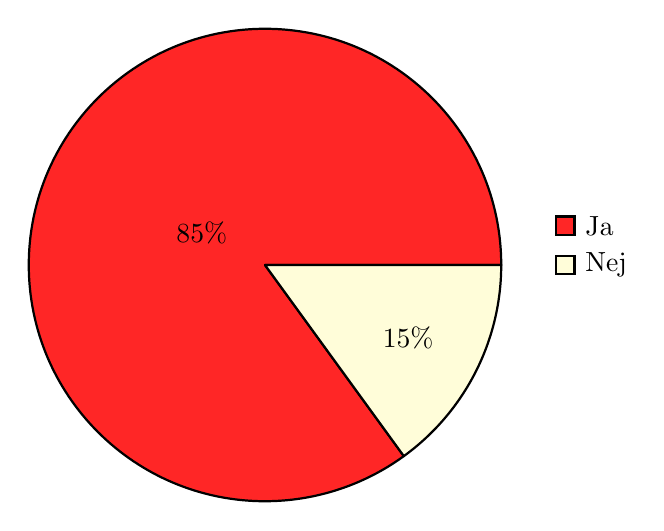
\begin{tikzpicture}
    \pie [text = legend, color={red!85, yellow!15}]{85/ Ja, 15/ Nej}
\end{tikzpicture}
    
\section{Teori}
    \label{sec:Teori}
    \input{Sections/Teori/Teori.tex}
    
    \subsection{Vad är ett problem?}
        %\textcolor{Mahogany}{Vi definierar ett problem som en uppgift som man på förhand inte vet hur man ska lösa. }

% Vad är inte problemlösning
\textcolor{green}{Begreppet problem är ett brett uttryck och hur det ska tolkas är inte självklart. En studie från Umeå universitet \cite{problemVarierandeDef} försökte man klargöra hur begreppet problem var tänkt att tolkas enligt Skolverkets läroplan och jämföra det med hur lärare faktiskt tolkade begreppet. I studien framkom det att Skolverket i sin läroplan inte uttryckligen definierade vad ett problem var och att lärarnas uppfattningar om vad ett problem var varierade stort. Denna bakgrund belyser alltså tydligt att det inte råder konsensus kring någon specifik definition om vad ett matematiskt problem är. Idag däremot har Skolverket en definition på sin webbplats och eftersom denna rapport handlar om matematiska problem för gymnasiet anser vi det lämpligt att i första hand titta på vad skolverket säger i frågan. De skriver följande~\cite{ProblemDef}:}

\begin{displayquote}
\textcolor{green}{Ett problem är en uppgift som inte är av standardkaraktär och kan lösas på rutin. Det innebär att varje frågeställning där det inte på förhand för eleven finns en känd lösningsmetod kan ses som ett problem.}
\end{displayquote}

\noindent\textcolor{green}{Denna definition belyser svårigheten med att kalla något för ett problem, nämligen att den uppgift som är ett problem för en person, kan vara en enkel standarduppgift för någon annan. Trots detta kommer vi benämna våra framtagna matematiska problem som just problem, eftersom de är gjorda för att vara nya och utmanande för gymnasielever.} 
\textcolor{green}{I detta arbete har vi valt att använda en något mer sammanfattad version av samma definition som Skolverket använder, nämligen att:}

\begin{displayquote}
\textcolor{green}{Ett problem är en uppgift som man inte på förhand vet hur man ska lösa.}
\end{displayquote}

\noindent %\textcolor{green}{Notera att detta betyder att en uppgift kan vara ett problem för någon, medan den för någon annan, med andra förkunskaper, är ett standardproblem.Notera också att detta innebär att vi i vissa sammanhang kommer kalla de uppgifter vi gör för just uppgifter, även om målet är att de ska vara problem för gymnasieeleverna.}

\textcolor{green}{Problemlösning i sin tur beskrivs enligt Skolverket som förmågan att kunna lösa ett problem. Vidare skriver de att~\cite{ProblemDef}:}

% vår definition av problemlösning:
% "En uppgift som man inte på förhand vet hur man ska lösa. Notera att dettabetyder att en uppgift kan vara ett problem för någon, medan den för någonannan, med andra förkunskaper, är ett standardproblem. Notera också att dettainnebär att vi i vissa sammanhang kommer kalla de uppgifter vi gör för justuppgifter, även om målet är att de ska vara problem för gymnasieeleverna."

%\noindent \textcolor{lila}{
 %   Denna definition gör det på sätt och vis mycket svårt att skapa ett problem, eftersom den innebär att en uppgift som är ett problem för en person, kan vara en ren standarduppgift för någon annan. Definitionen innebär också att problemlösning är ett mycket brett område. Nedan presenteras några viktiga delar som, tillsammans eller var och en för sig, kan lyftas fram i ett bra problem.
%}

\begin{displayquote}
\textcolor{green}{Problemlösningsförmåga innebär att kunna analysera och tolka problem vilket inkluderar ett medvetet användande av problemlösningsstrategier som att till exempel förenkla problemet, införa lämpliga beteckningar, ändra förutsättningarna. Att lösa problemet innebär att genomföra ett resonemang där grunderna för resultatets giltighet blir tydligt och resultatet korrekt.}
\end{displayquote}

\noindent \textcolor{green}{
Definitionen visar att problemlösning är ett mycket brett område.}
% Värt att notera är att om problemet anses vara löst så ska det inkludera ett resultat. Alltså påstår denna definition även något om ett problems egenskaper, nämligen att ett problem ska ha ett \textsl{korrekt resultat}. Detta är som sagt Skolverkets egna definition och ingen officiell definition. Lösningen av ett problem kan exempelvis handla om att göra approximationer eller optimeringar och därför vill vi hävda att ett problem nödvändigtvis inte behöver ha \textit{ett} korrekt resultat. I övrigt håller vi med Skolverkets beskrivning om problemlösningsförmåga och problemlösning.}

\textcolor{green}{Nedan presenteras några viktiga egenskaper som hör samman med problem och problemlösningsstrategier. Dessa egenskaper kan tillsammans, eller var och en för sig, lyftas fram i ett bra problem.}
%\textcolor{WildStrawberry}{
%    Komplexiteten med att definiera vad ett problem är ligger i att det existerar olika syften med vad ett problem vill få ut från den som testas. Vissa problem vill att du hittar x - kan du hitta x? Andra problem kanske inte har ett exakt svar - tillvägagångssättet när man försöker lösa problemet är det som är utvecklande. Det vi vill ta ställning för är att en ''lös ut x''-uppgift som är dekorerad i en \textit{saga} skapar inte ett intressant problem och kunde lika väl varit den vanliga ''vad är x''-övningen.
%}

% Vad är problemlösning
%\textcolor{WildStrawberry}{
%    Det finns en mängd olika infallsvinklar man kan ta för att definiera \textit{ett problem}. Den som testas bör behöva fundera på vad som är viktigt i en given situation och skapa egen modellering av verkligheten. Ett problem bör skapa ett behov för teorin som kan appliceras och därav förhoppningsvis härleda för en djupare förståelse till varför teorin fungerar. När man fått fundera på hur man \textit{kan} gå till väga för att lösa problem innan man får underlaget så binder man en starkare koppling till materialet och bör därför komma ihåg det bättre\todo{källa}. Men vi vill definiera att \textit{ett problem} är en form av uppgift där man får arbeta med en situation eller uppställning som man inte kan svaret till på förhand.
%}

\textcolor{lila}{
    Till att börja med kräver problemlösning ett \textsl{undersökande arbetssätt}. Det handlar om att analysera problemet och bryta ner det i mindre delar, och därefter hantera varje del var för sig. Ofta måste man prova sig fram med olika lösningsmetoder innan man hittar en som fungerar.
}
        
\textcolor{lila}{
    En vanlig form av problemlösning är också att använda \textsl{öppna problem}. Det innebär ett  problem till vilket det finns flera olika möjliga lösningsgångar för att hitta ett svar, och detta svar behöver inte heller vara unikt utan kan variera beroende på vilka antaganden som gjorts. Ett exempel på ett öppet problem är att man ska planera en pool med en viss volym, vilket självklart kan göras på en mängd olika sätt.
}

\textcolor{lila}{
    En annan viktig del är att kunna översätta ett problem till \textsl{matematiska modeller}. Detta är en nyttig förmåga att besitta i många olika sammanhang, även i arbetslivet~\cite{TheElephant}. Det är också minst lika viktigt att kunna granska en modell med kritisk blick, och fundera på i vilka sammanhang den gäller och när den leder till orimliga resultat.
}
\textcolor{Mahogany}{Inte minst så är det ett kunskapskrav för gymnasiematematiken att kunna tillämpa matematiska modeller, något som Skolverket beskriver som \textsl{modelleringsförmåga} \cite{ProblemDef} \cite{skolverketMatte}. Denna förmåga beskrivs som följande:}

\begin{displayquote}
    \textcolor{Mahogany}{
        \textsl{Modelleringsförmåga innebär att kunna formulera en matematisk beskrivning – modell – utifrån en realistisk situation.}
    }
\end{displayquote}
\noindent\textcolor{Mahogany}{Vidare beskrivs denna modelleringsförmåga som förmågan att kunna koppla resultatet till en verklig situation och bedöma ifall det är rimligt, för att sedan eventuellt utvärdera modellen på nytt.}
        
    \subsection{Diskussioner och kommunikation inom matematik}
        \textcolor{cyan} {
Givande diskussioner kan få elever att inse att det är tillåtet att ha egna idéer och tankar kring matematik, ett ämne som annars ofta upplevs handla om att följa regler. När elever diskuterar problem med varandra så lär de av varandra, och kan ofta uttrycka sig på ett sätt som kan göra det lättare för dem att förstå än vad ofta läraren kan.  \cite{TheElephant}
}

\textcolor{cyan} {
Faktum är att diskussion är så viktigt för bra problemlösning att Hagland, Hedrén och Taflin skriver att den viktigaste skillnaden mellan ett vanligt problem och vad de kallar ett rikt problem är att det rika problemet leder till diskussion. \cite{RikaProblem}
}

\textcolor{cyan} {
Även Skolverket lyfter att matematikundervisning där elevers egna lösningstratergier diskuteras leder till mycket positiva resultat och ökar elevers lust att lära. \cite{Skolverket03}
}

\textcolor{cyan} {
Ett land som tas upp som ett exempel på god matematikundervisning av både Skolverket och Boaler är Japan \cite{TheElephant}. I Japan läggs stor vikt vid att efter eleverna löst ett problem så ska de dela med sig utav sina lösningar och diskutera dem med varandra. Diskussionen används som en utgångspunkt för att läraren ska kunna lyfta viktiga aspekter ur deras lösningar och tillvägagångsätt. \cite{Skolverket03}
}
%Rika problem är problem som leder till diskussion  

%Ger chans att lyfta sina egna idéer och utveckla dem. 

%Diskussion leder till öka lust att lära. 

%Japanska skolan lägger fokus på diskussion och lyfts som ett föredöme av både skolverket och Jo Boaler 

% Tar upp strukturen med diskussion före och efter elever får lösa problemet. 
        
    \subsection{Arbeta i grupp}
        \textcolor{cyan} {
Att låta elever arbeta med problemlösning i små grupper om två till fyra personer leder till att varje elev ges möjlighet att diskutera och reflektera angående problemet. Eleverna får prata om sina idéer till lösningar, lyssna på andra elevers idéer, samt även ges möjlighet att fråga, kritisera och bemöta kritik på ett positivt sätt. När eleverna får förklara sina tankar leder till ökad matematiksförståelse. \cite{RikaProblem}
}

\textcolor{cyan} {
Som tidigare nämnts i \ref{sec:Gruppindelning} är det vanligt att skolor delar in elever i grupper efter deras matematikfärdigheter, dock hävdar både Boaler och Rika Problem att det är bättre med heterogena grupper vad det gäller matematikkunskap \cite{TheElephant}\cite{RikaProblem}. Boaler skriver att klassrum där elever med olika förkunskaper jobbar med varandra med metoder anpassade för att alla elever ska lära av varandra är mer rättvisa\cite{TheElephant}. 
}

\textcolor{cyan} {
Rika problem rekommenderar att läraren blandar medelpresterande elever med högepresterande eller lågpresterande elever när man gör gruppindelningen, men varnar samtidigt för att inte göra grupperna extremt homogena eller heterogena\cite{RikaProblem}.
}

% I blandade grupper hjälper elever varandra vilket leder till fina ord som equality och allt blir bättre - Jo Boaler

% Även Rikaproblem rekommenderar att man blandar medelpresterande elever med högepresterande eller lågpresterande elever när man gör grupp indelningen, men varnar samtidigt för att inte göra grupperna extremt homogena eller heterogena. 


\textcolor{cyan} {
En negativ aspekt med grupparbete är att vissa elever kan bli sittande passivt medan resten av gruppen löser uppgiften åt dem. \cite{RikaProblem} %Ta upp att det blir värre ju fler man blir på någotsätt? 
}

%Bygga en rödtråd till förra kapitlet genom Japanska skolan. 



% Problemlösning i grupp anses vara roligare än vanliga mattelektion - Skolverket

% Saknas något om olika gruppstorlekar, samt nackdelar

% En studie visar att 2 är bättre än 1 förrutom för de allra bästa eleverna där det är ungefär lika bra, men 3-5 är strängt bättre. Den säger även att testpersonerna hade något roligare när det arbetade individuellt.

%Negativt - Om man börjar med grupparbete så kan vissa elever bli sittande passivt medan resten av gruppen löser uppgiften åt dem. - Rikaproblem



% Grupper bör ligga på 2-4 elever, eftersom det i en sådan grupp ger alla elever möjlighet att delta i diskussioner - Rika problem 

% Gruppering efter färdigheter är vanligt, enligt skolverket. 
        
    \subsection{Programmering och matematik}
        \textcolor{Mahogany}{Att lära sig programmera är inte bara att lära sig ett programmeringsspråks syntax. Framförallt så är det att kunna bryta ner ett problem i mindre delar, i datasammanhang även kallat \textsl{subrutiner}, och definiera tydliga steg för hur man genomför dessa. Att få träning och efter hand färdighet för detta gör att man med större sannolikhet kommer att kunna bemöta ett nytt problem på ett mer systematiskt och rationellt sätt, oavsett om det är relaterat till programmering eller inte.}

\textcolor{Mahogany}{Eftersom en dator behöver exakta instruktioner och inte själv har förmåga att tolka vad som är rätt och fel så är det viktigt att man är tydlig med vad man menar att ett program ska göra. Vad en dator däremot är bra på är att utföra dessa instruktioner på väldigt mycket kortare tid än vad människor kan. Detta ger ett väldigt kraftfullt verktyg för många saker, faktum är att detta används i så stor utsträckning att vårt moderna samhälle still stor del är beroende av det. Det kan handla om att kunna betala sina räkningar på internetbanken på ett säkert sätt till att hitta ett lunchställe i en ny stad med hjälp av sökmotorer.}

\textcolor{Mahogany}{
    Kunskap i programmering är mer efterfrågad i samhället idag än någonsin tidigare. Att lära sig programmera är också en möjlighet för elever att med relativt fria tyglar få syssla med problemlösning. Detta är något som man har väldigt stor nytta av i matematik~\cite{TheElephant}, och som matematik i stor utsträckning även går ut på. Som vi nämnt i~\ref{sec:Forandringar} så kommer programmering framöver även ingå i kursplanen för gymnasiematematik. Detta gör det väldigt aktuellt att inkludera matematikrelaterade programmeringsuppgifter i vårt projekt, och de flesta av de programmeringsuppgifter som vi tagit fram har en tydlig koppling till matematiken.
}
        
    \subsection{Info om React?}
        
\section{Syfte}
    \subsection{''Mattedelen''}
    (Skriva om syftet med problemen, även varför vi riktar oss mot just gymnasiet.)
    \subsection{Hemsidans utvecklingsmiljö}
        \textcolor{Mahogany}{Hemsidan är ett sätt att förmedla de problem som vi utformat till fler än de som vi testar problemen med genom att göra det mer lättillgängligt att ta del av problemen. Med hjälp av denna kan vi ge lärare möjligheten att ta del av våra problem när de vill och känner att de har tid över. Det hjälper oss också att få spridning på problemen som vi utformat. Kanske tyckte de att problemen var givande och delar med sig av sidan till en kollega, som kanske i sin tur gör samma sak. I slutändan så hoppas vi helt enkelt att så många som möjligt kan ha hjälp av de problem som vi utformat.}

\textcolor{Mahogany}{Hemsidan är också det som kommer att leva kvar efter projektet, så vi har valt att inkludera en kort beskrivning om oss och vårt arbete, samt en liten informativ text till lärare med vad vi vill uppnå med våra problem och hur vi tänkt att de bör utföras.}

\section{Metod}

    \subsection{Skapandet av problemen}
        % Ta ställning till omständigheter
\textcolor{Mahogany}{Något som är viktigt att ta ställning till när man utformar problem för gymnasiematematik är att det måste vara förenligt med övriga undervisningen. Man ska övertyga både lärare och elever att det för det första är relevant, men också att det kommer att vara mer givande än att räkna i boken. Det är också viktigt att ha som en röd tråd vad man egentligen vill att elever ska få ut av ett problem, och försöker förmedla detta på ett naturligt sätt. Är problemlösning bara något som tar tid från räkning i boken eller kan man få elever att förstå att de kan gynnas av denna typ av matematikundervisning? Ett ''bra'' problem bör rimligtvis lyfta fram den nyttan. Framför allt så bör de även vara roliga att lösa.}

% Hur bör det utföras?
\textcolor{Mahogany}{Vi har lagt ner en del tid på att informera lärare hur vi tänker att våra problem ska utföras. Detta är för att vi vill att man ska få ut så mycket som möjligt från problemen framförallt via diskussion och reflektion. Diskussionsdelen är också ett sätt för elever att våga försöka lösa ett problem som till synes kanske skulle vara avskräckande. Oavsett svårighetsgraden på problemet så anser vi att diskussionen är en viktig del i lärandet, då man får möjligheten att uttrycka sin nivå av förstående och ens kunskap testas genom att man behöver förklara det för någon annan. Samtidigt så gynnas de elever som inte kommit lika långt att få höra hur andra tänkt, och därifrån kunna arbeta vidare själva.}

% Rimlig nivå
\textcolor{Mahogany}{En svårighet med att utveckla problem är att sätta en rimlig svårighetsgrad, speciellt med tanke på att vi under utvärderingen fick jobba med framför allt väldigt specifik tidsram. Ett sätt att konfrontera detta är att ha en tydlig grund som problemet bygger på, för att sedan möjliggöra vidareutveckling i största mån. Denna vidareutveckling handlar ofta om fördjupningsfrågor som uppmanar till diskussion, vilket kan underbygga elevernas möjlighet att få en djupare förståelse för ämnet.}
    
    \subsection{Test av problemen}

    \subsection{Hemsidan och latexponering}
        \textcolor{green}{Hemsidan utvecklades i programmeringsspråket Javascript. Fördelarna med att använda sig av ett programmeringsspråk som Javascript istället för att exempelvis bara använda HTML är att man kan designa sidan på många fler sätt och får total kontroll över sidans innehåll. Med total kontroll menas det att man skulle kunna ha annan material på webbplatsen än bara text- och bildmaterial. Det skulle kunna vara någon form av digitalt verktyg, t ex ett matematiskt problem som använder sig av en simulator. Detta kan göras med hjälp av Javascripts många olika bibliotek.}

\textcolor{green}{Biblioteket som användes för att utveckla webbplatsen var React JS. React JS är ett av de mest populära biblioteken att bygga webbplatser med i Javascript [källa]. I Reacts bibliotek finns främst verktyg för att jobba med vy-delen av en hemsida. Vill man integrera tyngre applikationer i webbsidan så finns möjligheter för det. Men om vyn är det största fokuset så är React ett mycket lämpligt val då det är väldokumenterat och gör det enkelt att bygga vidare på hemsidans design.}

    
\section{Resultat}

    \subsection{De problem som vi skapat}
    
    \subsection{Hemsidan}
        \textcolor{Mahogany}{Hemsidans design har gjorts enkel där känslan ska vara att man hela tiden är på ''en'' sida. Den består av olika problem som listas i ett rutnät på ''Problem''-sidan, innehållandes titel och bild. Klickar man på ett av problemen i rutnätet så kommer man vidare till en mer detaljerad vy över problemet med en kort beskrivande text följt av en länk till det fullständiga problemet. I många fall bifogas även en tillhörande PowerPoint, som är tänkt att underlätta utförandet. För programmeringsuppgifterna så bifogas även ett lösningsförslag skrivet i Java.}

\textcolor{Mahogany}{Hemsidan har även en startsida som designats för att kännas inbjudande och engagerande, där besökaren ges en introducerande text om vad vi arbetar med samt en knapp som tar personen direkt till problemen. Dessa kommer man givetvis också åt via menyn, skillnaden är att vi vill fånga uppmärksamheten på ett mer välkomnande sätt för den som besöker hemsidan för första gången genom att ha en knapp över en bild som illustrerar några av våra problem.}

\textcolor{Mahogany}{Till sist så inkluderas sidan ''Om oss'', som beskriver projektets arbete, samt en sida med ''Information till läraren'', vars innehåll beskrivs närmare i \ref{sec:Skapandetavproblem}.}

\section{Utfall}
    \label{sec:Utfall}
    \begin{itemize}
\item Hur problemen togs emot av lärare och elever
\item Att det fanns ett stort intresse i början av att testa uppgifterna, men att många hoppade av pga tidsbrist i samband med de nationella proven.
\end{itemize}


\section{Diskussion}

    \subsection{Hur vi kan påverka}
        % \textcolor{Mahogany}{
%     Som nämndes i avsnitt~\ref{sec:slutenkat} så var det under utvärderingen inte ovanligt att lärare kände att de inte hade tid att testa våra problem på grund av annat i kursplanen så som nationella prov. De var dock intresserade, och de flestakommenterade att problemen och uppläggen verkade bra. Vi hoppas därför att även om många lärare just nu inte kan utvärdera våra problem att vi ändå lyckats förmedla nyttan med denna typ av arbetssätt och att matematik bör handla mer om den undersökande delen som till större del bygger på diskussion och rimlighetsanalyser.
% }

\textcolor{Mahogany}{
    I \ref{sec:MerProblemlosning} så framgår det att många lärare påpekar att de anser problemlösning vara viktigt. Samtidigt känner de att de inte kan arbeta med det till den grad de skulle vilja på grund av tidsbrist, både på och inför lektionerna, och för att de inte vet hur man skulle göra det på ett bra sätt. De tyckte bland annat att det var svårt att hitta bra problem som är utmanande för hela klassen. %I utformandet av våra problem så försökte vi i någon mån att anpassa problemen efter vissa nivåer, kanske främst för testningssyften då vissa lärare uttryckte intresse av att testa problem som specifikt skulle passa in på en viss matematikkurs. Vi hade egentligen som utgångspunkt att utforma \textsl{bra} problem, utan hänsyn till vilken nivå den hamnar på. Samtidigt kan det vara bra att ta försöka få in vissa element som gör att man kan fånga upp relevant teori, eller efterfrågan av den, även om fokus fortfarande ligger på problemlösning.
}

    \textcolor{lila}{Med den fullständiga lektionsplanering som följer med hoppas vi kunna avlasta lärarna från en del av det förberedande arbete som krävs för att genomföra en problemlösningslektion, och därmed förbättra deras arbetssituation. Med den brist på lärare som råder idag är det viktigt ur ett samhällsperspektiv att spara på de resurser vi har, för att kunna utnyttja deras fulla potential genom att de får finnas till hands och handleda problemlösningen. Bristen av ren lektionstid är svårt för oss att påverka, men dels har vi även tryckt på den bevisade nyttan av problemlösning och dels hoppas vi som sagt att detta ska hjälpa med en del av de nuvarande faktorer som motverkar mer problemlösning i undervisningen.}
    
    \textcolor{lila}{Även om man arbetar hårt för att ändra matematikundervisningen, och utvecklingen enligt oss är på väg åt rätt håll, så tror vi att det finns mer som kan göras för att hjälpa den på traven. Vi vill därför arbeta för att hjälpa lärarna att få eleverna att gå från att beskriva matematiken som ''tråkig'' och ''onödig'' och istället börja använda ord som ''rolig'', ''spännande'' och ''användar''. Kanske till och med ''kreativ''.}
    
% \textcolor{Mahogany}{
%     Vi hoppas att även om det är en småskalig inverkan så kan vi fortfarande hjälpa till att förändra bilden kring matematik så att den inte ska förknippas med ord som och att elever ska känna att det är något kreativt och undersökande snarare än att handla om memorering och upprepning.}
    %\textcolor{lila}{Och även om detta bara är en liten del av den utveckling vi hoppas följer, så hoppas vi att matematikundervisningen utvecklas till en mer levande och kreativ process. I bästa fall leder detta till en ny generation av skickliga problemlösare, som kan säkra Sveriges roll i framtidens tekniska samhälle. 
%}
    
    \subsection{Vad är ett bra problem?}
        % Vi testade bara problem som utfördes under 1h
\textcolor{Mahogany}{
    %Målet med de problem som vi utformat i projektet är att framhäva vikten av problemlösning i matematiken. Samtidigt så är också ett mål att visa hur den kan vara användbar, och att den användbarheten inte enbart existerar i det ''matteland'', som beskrivs i \ref{sec:Verklighetsanknytning}.  Man vill inte heller, som nämndes i avsnitt~\ref{sec:problemdef}, riskera att verklighetsanknytning blir en alltför stor faktor i problemskapandet. Ibland kan ett abstrakt problem leda till ett större engagemang och nyfikenhet som ett med en tydlig verklighetsanknytning. En utmaning med att utforma verkliga problem är därför att ta ställning till detta samtidigt som man framhäver den mångsidiga nyttan av matematiken.
    Ett mål med de problem som vi har utformat är att vi vill visa hur användbar matematik kan vara, och att den användbarheten inte enbart existerar i det ''matteland'', som beskrivs i \ref{sec:Verklighetsanknytning}.  Man vill inte heller, som nämndes i avsnitt~\ref{sec:problemdef}, riskera att verklighetsanknytning blir en alltför stor faktor i problemskapandet. Ibland kan ett abstrakt problem leda till ett större engagemang och nyfikenhet som ett med en tydlig verklighetsanknytning. En utmaning med att utforma verkliga problem är därför att ta ställning till detta samtidigt som man framhäver den mångsidiga nyttan av matematiken.
}

%\textcolor{Mahogany}{
    % Detta kan vara betydligt lättare att uppnå med programmeringsproblem, då man, utöver programmeringsspråkets syntax, inte är bunden till hur man kan lösa något av problemen. Man ges också i många fall möjligheten att själv avgränsa hur utförligt problemet ska utföras. Som exempel så har vi utformat ett problem där man ska verifiera ett personnummer, där man företrädesvis kan använda sig av den så kallade Luhn-algoritmen\cite{Luhn}. Dock så kanske det inte räcker med att enbart kontrollera med hjälp av den algoritmen. Om man kontrollerar personnummer på de i sin klass så kanske man vill kontrollera att personen inte är född på 1800-talet exempelvis!
%}
 
% Röd tråd samt övertyga elever att det är relevant
\textcolor{Mahogany}{
    Med våra uppgifter vill vi övertyga både lärare och elever att de är relevanta, men också att de kommer vara mer givande än att enbart räkna i boken. Det är också viktigt att ha som en röd tråd vad man egentligen vill att elever ska få ut av ett problem, och försöka förmedla detta på ett naturligt sätt. Är problemlösning bara något som tar tid från räkning i boken eller kan man få elever att förstå att de kan gynnas av denna typ av matematikundervisning? Ett bra problem bör därför rimligtvis lyfta fram den nyttan. Framför allt så bör problemen även vara roliga att lösa, och ge eleverna en chans att utforska och utmanas av matematiken.
}

% Hur bör det utföras?
\textcolor{Mahogany}{
    Vi har lagt ner en del tid på att informera lärare hur vi tänker att våra problem ska utföras. Detta framförallt för att vi anser att diskussion och reflektion är mycket viktiga för inlärningen, vilket även diskuterades i avsnitt~\ref{sec:Diskussion}. Diskussionsdelen är också ett sätt för elever att våga försöka lösa ett problem som till synes kanske skulle vara avskräckande. Oavsett svårighetsgraden på problemet så anser vi att diskussionen är en viktig del i lärandet, då man får möjligheten att uttrycka sin nivå av förstående och ens kunskap testas genom att man behöver förklara det för någon annan. Samtidigt så gynnas de elever som inte kommit lika långt av att få höra hur andra tänkt, och därifrån kunna arbeta vidare själva.
}

% Rimlig nivå
\textcolor{Mahogany}{
    En svårighet med att utveckla problem är att sätta en rimlig svårighetsgrad, speciellt med tanke på att vi under utvärderingen fick jobba med en väldigt specifik tidsram. Ett sätt att konfrontera detta är att ha en tydlig grund som problemet bygger på, för att sedan möjliggöra vidareutveckling i största mån. Denna vidareutveckling handlar ofta om fördjupningsfrågor som uppmanar till diskussion, vilket kan underbygga elevernas möjlighet att få en djupare förståelse för ämnet.
}
        
    \subsection{Problemlösning}
        % Om det finns något här som ni vill ha med i rapporten så är det bara att plocka, men personligen så kände jag att det här inte längre tillförde något.

\textcolor{Mahogany}{
    Från svaren på en av våra undersökningsenkäter så märkte vi att begreppet problemlösning skiljde sig från lärare till lärare, där vissa kände att räkning i boken var problemlösning. Det är dock inte ett helt självbeskrivande begrepp som med fördel kan förtydligas.
}

\textcolor{Mahogany}{
    Även om problemlösning är en del av kursplanen i matematik så är det tydligt att det skiljer sig i vilken utsträckning och form det utövas. Som nämnts i \ref{sec:Forandringar} så ska problemlösning vara både ett mål och medel i undervisningen enligt kursplanen för gymnasiematematik, dessvärre så förlitar sig lärare i stor utsträckning enbart på de problem som kursboken tillhandahåller. Därtill blir den typen av problem ofta enbart extrauppgifter för de som hinner \cite{2010UndervisningenGymnasieskolan}. Det är alltså rimligt att anta att problemlösning i gymnasiematematik är bristfällig samt att lärare behöver fler verktyg och resurser för att uppnå dessa mål.
}

\textcolor{Mahogany}{
    Vi tror att en stor del handlar om att låta elever få diskutera med varandra, men utformningen av rätt typ av problem är givetvis också viktigt. Det ska inte mynna ut till att handla om att ta ur värden och sedan applicera dessa på aktuell teori som nyss gåtts igenom. Men det gäller också att ge lärare resurserna och samtidigt utmana deras uppfattning om vad problemlösning är, för att på så sätt kunna öka andelen av vad vi ser som problemlösning.
    Kanske är en stor anledning att det inte är mer problemlösning i undervisningen att lärare i olika utsträckning är osäkra på hur de ska genomföra en sådan undervisning, med en kombination av att inte ha rätt resurser. Frågan är om man uteslutande kan förlita sig på att enbart kursböckerna ska täcka denna del av kursplanen, men samtidigt krävs tid och resurser om man vill förbättra detta, något som många lärare känner att de inte har.
}
    
    \subsection{Hemsida}
        % Just att ha en plats där vem som helst kan ha åtkomst till problemen anser vi är viktigt. När möjligheten finns att kunna dela information på ett lättillgängligt sätt, då når man potentiellt ut till fler lärare som skulle vara intresserade utav att testa problemen.

% Motargumentet till att bygga en hemsida är att vi skulle kunna skicka ut PDF-filer per epost till lärare - vilket var fallet när vi testade problemen. Men potentialen för spridning blir mycket enklare med möjligheten att klistra in en länk i ett mail, chattrutor eller sociala nätverk än att först ladda ner en fil och sedan bifoga den. Tanken är att ju fler handlingar som finns i en interaktion, ju större chans är det att man missar engagemangen att dela med sig till vänner och kollegor som potentiellt skulle vilja testa.

\section{Slutsats}

\newpage
\begin{thebibliography}{3}
        %Skriv källa:
    %1
    \bibitem{Ignacio&Barona}
    N.G. Ignacio, L.J.B.N.a.E.G. Barona, "The Affective Domain in Mathematics Learning," i \textsl{IEJME-Mathematics Education}. [Online]. Tillgänglig: \url{http://iejme.com/makale/70}. Hämtad: 5 apr 2017.
    
    %2
    \bibitem{Skolverket03}
    Skolverket, ''Lusten att l{\"a}ra : med fokus p{\aa} matematik : nationella kvalitetsgranskningar 2001-2002'',  Skolverket, Stockholm, Skolverkets rapport, 1103-2421 ; 221, 2003
    
    %Rapportserie och nummer, volym, år. [Online]. Tillgänglig: \url{http://www.mah.se/pages/45519/lustattlara.pdf}. Hämtad: datum.
   
    % Author(s). Book title. Location: Publishing company, year, pp. 
    % http://libris.kb.se/bib/8904038?vw=full
    
    %3
    \bibitem{CompareOECD}
    “Compare your country - PISA 2015,” Compare your country by OECD. [Online]. Tillgänglig: http://www.compareyourcountry.org/pisa/country/SWE. Hämtad: Feb. 10, 2017.
    
    %4
     \bibitem{traditionellMatte}
    E. Berggren, "Traditionell skolmatematik: En studie av undervisning och lärande under en matematiklektion," examensarbete, Institutionen för datavetenskap, fysik och matematik, Linnéuniversitetet, Växjö, Sverige, 2010. [Online]. Tillgänglig: \url{http://www.diva-portal.org/smash/get/diva2:337889/FULLTEXT01.pdf}. Hämtad: 7 mars, 2017.
    
    %5
    \bibitem{TheElephant}
    J. Boaler, ''The Elephant in the Classroom: Helping Children Learn and Love Maths,'' 
    London,
    England: Souvenir Press Ltd, 
    2010. 
    
    %6
    \bibitem{Nämnaren}
    E. Silver, M. Smith, "Samtalsmiljöer," Nämnaren, nr. 1, ss. 55-59, feb. 2015. [Online]. Tillgänglig: \url{http://ncm.gu.se/pdf/namnaren/5559_15_1.pdf}. Hämtad: Apr. 4, 2017
    
    %7
    \bibitem{2016Senare}
    ''Senare matematik i gymnasieskolan (matematik 3c),'' Startsidan - Skolinspektionen. [Online]. Tillgänglig: \url{https://www.skolinspektionen.se/sv/Beslut-och-rapporter/Publikationer/Granskningsrapport/Kvalitetsgranskning/senare-matematik-i-gymnasie-skolan-matematik-3c/}. Hämtad: Feb. 10, 2017.
    
    %8
    \bibitem{2010UndervisningenGymnasieskolan}
    “Undervisningen i matematik i gymnasieskolan,” Startsidan - Skolinspektionen. [Online]. Tillgänglig: \url{https://www.skolinspektionen.se/sv/Beslut-och-rapporter/Publikationer/Granskningsrapport/Kvalitetsgranskning/------Undervisningen-i-matematik-i-gymnasieskolan/}. Hämtad: Feb. 10, 2017.
    
    %9
    \bibitem{lockhart}
    P. Lockhart, \textit{A mathematician's lament}. New York: Bellevue Literary Press, 2009.
    
    %10
    \bibitem{GY00-GY11}
    Skolverket, ''Jämförelse med kursplan 2000,'' 2011. [Online]. Tillgänglig: \url{https://www.skolverket.se/laroplaner-amnen-och-kurser/gymnasieutbildning/gymnasieskola/mat}. Hämtad: Apr. 11, 2017.
    
    %11
    \bibitem{regeringen}
    Regeringskansliet, ''Stärkt digital kompetens i läroplaner och kursplaner,'' \textsl{regeringen.se} 2017. [Online]. Tillgänglig: \url{http://www.regeringen.se/pressmeddelanden/2017/03/starkt-digital-kompetens-i-laroplaner-och-kursplaner/}. Hämtad: Apr. 11, 2017.
    
    %12
    \bibitem{itiskolan}
    ?
    M. Halápi, K.L. Rüter, ''Redovisning av uppdraget om att föreslå nationella IT-strategier för skolväsendet'', Skolverket,
    
    \url{https://www.skolverket.se/om-skolverket/publikationer/visa-enskild-publikation?_xurl_=http\%3A\%2F\%2Fwww5.skolverket.se\%2Fwtpub\%2Fws\%2Fskolbok\%2Fwpubext\%2Ftrycksak\%2FBlob\%2Fpdf3647.pdf\%3Fk\%3D3647}
    
   %13
   \bibitem{prog_utbildning}
   Skolverket, ''Tydligare om digital kompetens i läroplaner, kursplaner och ämnesplaner'', 2017. [Online]. Tillgänglig: \url{https://www.skolverket.se/skolutveckling/resurser-for-larande/itiskolan/styrdokument}. Hämtad: Apr. 11, 2017.
   
   %14
   \bibitem{RikaProblem}
    Hagland, K., Hedrén, R. and Taflin, E., \textit{Rika matematiska problem - inspiration till variation}, Malmö, Sverige, Elanders Berlings AB, 2005.
\end{thebibliography}
\end{document}